\documentclass{beamer}
%%%%%%%%%%%%%%%%%%%%%%%%%%%%%%%%%%%%%%%%%%%%%%%%%%%%%%%%%%%%%%%

% Define packages
\usepackage{beamerthemesplit}
\usepackage{graphicx,amsfonts,psfrag,layout,subcaption,array,longtable,lscape,booktabs,dcolumn,natbib,amsmath,amssymb,amssymb,amsthm,setspace,epigraph,chronology,color, colortbl,caption}
\usepackage[]{graphicx}\usepackage[]{color}
\usepackage[page]{appendix}
\usepackage{hyperref, url} %For submission, uncheck and fix URLs ($$)
\usepackage[section]{placeins}
\usepackage[linewidth=1pt]{mdframed}

% Footnotes stick at the bottom
\usepackage[bottom]{footmisc}

% New footnote characters
\usepackage{footmisc}
\DefineFNsymbols{mySymbols}{{\ensuremath\dagger}{\ensuremath\ddagger}\S\P
   *{**}{\ensuremath{\dagger\dagger}}{\ensuremath{\ddagger\ddagger}}}
\setfnsymbol{mySymbols}

% New tabular environment
\usepackage{tabularx}
\newcolumntype{Y}{>{\raggedleft\arraybackslash}X}% raggedleft column X

% Define appendix 
\renewcommand*\appendixpagename{Appendix}
\renewcommand*\appendixtocname{Appendix}

% Position floats
\renewcommand{\textfraction}{0.05}
\renewcommand{\topfraction}{0.95}
\renewcommand{\bottomfraction}{0.95}
\renewcommand{\floatpagefraction}{0.35}
\setcounter{totalnumber}{5}

% Colors for highlighting tables
\definecolor{Gray}{gray}{0.9}

% Different font in captions
\newcommand{\captionfonts}{\scriptsize}

\makeatletter  % Allow the use of @ in command names
\long\def\@makecaption#1#2{%
  \vskip\abovecaptionskip
  \sbox\@tempboxa{{\captionfonts #1: #2}}%
  \ifdim \wd\@tempboxa >\hsize
    {\captionfonts #1: #2\par}
  \else
    \hbox to\hsize{\hfil\box\@tempboxa\hfil}%
  \fi
  \vskip\belowcaptionskip}
%\makeatother   % Cancel the effect of \makeatletter
 
% Number assumptions
\newtheorem*{assumption*}{\assumptionnumber}
\providecommand{\assumptionnumber}{}
\makeatletter
\newenvironment{assumption}[2]
 {%
  \renewcommand{\assumptionnumber}{Assumption #1}%
  \begin{assumption*}%
  \protected@edef\@currentlabel{#1}%
 }
 {%
  \end{assumption*}
 }
\makeatother

% Macros
\newcommand{\Adv}{{\mathbf{Adv}}}       
\newcommand{\prp}{{\mathrm{prp}}}                  % How to define new commands 
\newcommand{\calK}{{\cal K}}
\newcommand{\outputs}{{\Rightarrow}}                
\newcommand{\getsr}{{\:\stackrel{{\scriptscriptstyle\hspace{0.2em}\$}}{\leftarrow}\:}}
\newcommand{\andthen}{{\::\;\;}}    %  \: \; for thinspace, medspace, thickspace
\newcommand{\Rand}[1]{{\mathrm{Rand}[{#1}]}}       % A command with one argument
\newcommand{\Perm}[1]{{\mathrm{Perm}[{#1}]}}       
\newcommand{\Randd}[2]{{\mathrm{Rand}[{#1},{#2}]}} % and with two arguments
\newcommand{\E}{\mathrm{E}}
\newcommand{\Var}{\mathrm{Var}}
\newcommand{\Cov}{\mathrm{Cov}}
\DeclareMathOperator*{\plim}{plim}
\newcommand{\ind}{\mathbb{I}} % Indicator function
\newcommand{\pr}{\mathbb{P}} % Generic probability
\newcommand{\ex}{\mathbb{E}} % Generic expectation
\newcommand{\cov}{\mathrm{Cov}}
\newcommand\independent{\protect\mathpalette{\protect\independenT}{\perp}}
\def\independenT#1#2{\mathrel{\rlap{$#1#2$}\mkern2mu{#1#2}}}
\newcommand{\possessivecite}[1]{\citeauthor{#1}'s [\citeyear{#1}]} 

% Making a DAG
\usepackage{tkz-graph}  
\usetikzlibrary{shapes.geometric}
\tikzstyle{VertexStyle} = [shape            = ellipse,
                               minimum width    = 6ex,%
                               draw]
 \tikzstyle{EdgeStyle}   = [->,>=stealth']      


%color
\usecolortheme[RGB={50,200,50}]{structure} 

\usetheme[secheader]{Boadilla} 
\setbeamertemplate{items}[default] 
\setbeamercovered{transparent}
\setbeamertemplate{blocks}[rounded][shadow=true] 
\setbeamertemplate{navigation symbols}{} 
\mode<presentation>
\title[]{Estimating population average treatment effects from experiments with noncompliance}

\author[K. Ottoboni, J. Poulos]{Kellie Ottoboni, Jason Poulos}
\institute[]{Stat 215B}
\date[04/30/15]{April 30, 2015}
\begin{document}

\frame{\titlepage}

\section[Introduction]{}

\begin{frame}
\frametitle{Motivation}
\begin{itemize}
\item RCTs are the ``gold standard'' for estimating the causal effect of a treatment
\begin{itemize}
\item External validity is an issue when RCT participants don't reflect the target population
\item Non-compliance to treatment assignment biases estimates of the sample average treatment effect (SATE) towards $0$
\end{itemize}
\item Idea: reweight responses in the treatment group of RCT compliers to estimate population average treatment effect on the treated (PATT)
\begin{itemize}
\item \cite{Hartman} develop a nonparametric reweighting method to extend SATE to PATT
\item We extend this method to the case of one-way crossover
\end{itemize}
\end{itemize}
\end{frame}

\section[Estimation]{}

\begin{frame}
\frametitle{Estimating treatment effects}
\begin{itemize}
\item Neyman-Rubin framework: each $i = \left\{1, ..., N \right\}$ participants have four potential outcomes, $Y_{ist}$ for $s = 0,1$ and $t = 0,1$
\begin{itemize}
\item S = study assignment: S=1 for RCT, S=0 for population/observational study
\item T = treatment assignment: T = 1 for treatment, T = 0 for control
\item D = treatment received
\end{itemize}
\item Other variables
\begin{itemize}
\item W = observed covariates
\item C = compliance to treatment
\item Y = response
\end{itemize}
\end{itemize}
\end{frame}


\begin{frame}
\frametitle{Estimating treatment effects}
\begin{figure}[h]
\begin{tikzpicture}[scale=1.25] 
\SetGraphUnit{2} 
\Vertex{W}  \NOEA(W){S} \EA(S){T}  \EA(W){C} \SOEA(T){D} \SOEA(C){Y} \SOWE(D){Y}
\Edges(W, S, T) \Edges(W,T) \Edges(W, C) \Edges(T, D) \Edges(C, D) \Edges(W, Y) \Edges(D, Y)
\end{tikzpicture}
\caption{Causal diagram indicating the conditional independence assumptions needed to estimate the PATT.}\label{fig:DAG}
\end{figure}

\end{frame}

\begin{frame}
\frametitle{Estimating treatment effects (cont.)}
\begin{assumption}{1}{}\label{consistency}
Consistency under parallel studies: for all $i$ and for $t=0, 1$,
$$Y_{i0t} = Y_{i1t}$$
\end{assumption}
\end{frame}

\begin{frame}
\frametitle{Estimating treatment effects (cont.)}
\begin{assumption}{2}{}\label{si_treat}
Strong ignorability of sample assignment for treated:
\begin{equation*}
(Y_{01}, Y_{11}) \independent S \mid (W, T=1,C = 1), 0 < \pr(S=1 \mid W, T=1,C = 1) <1 
\end{equation*}
\end{assumption}
\noindent Potential outcomes for treatment are independent of sample assignment for individuals with the same covariates $W$ and assignment to treatment.

\begin{assumption}{3}{}\label{si_ctrl}
Strong ignorability of sample assignment for controls:
\begin{equation*}
(Y_{00}, Y_{10}) \independent S \mid (W, T=1,C = 1), 0 < \pr(S=1 \mid W, T=1,C = 1) <1 
\end{equation*}\end{assumption}

\noindent Potential outcomes for control are independent of sample assignment for individuals with the same covariates $W$ and assignment to treatment.
\end{frame}

\begin{frame}
\frametitle{Estimating treatment effects (cont.)}
\begin{assumption}{4}{}\label{sutva}
Stable unit treatment value assumption (SUTVA):
\begin{equation*}
Y_{ist}^{L_i} = Y_{ist}^{L_j},  \forall i \neq j
\end{equation*}
where $L_j$ is the treatment and sample assignment vector for unit $j$. \end{assumption}
 
\begin{assumption}{5}{}\label{compl}
Conditional independence of compliance and assignment:
\begin{equation*}
C \independent T=1 \mid W, 0 < \pr(C = 1 \mid W) < 1
\end{equation*}
\end{assumption}
\end{frame}

\begin{frame}
\frametitle{Estimating treatment effects (cont.)}
\begin{assumption}{6}{}\label{monotonicity}
Monotonicity: 
\begin{equation*}
T_i \geq D_i, \forall i
\end{equation*}
\end{assumption}
\noindent This assumption implies that there are no defiers and that crossover is only possible from treatment to control.
\begin{assumption}{7}{}\label{ER}
Exclusion restriction: For non-compliers
\begin{equation*}
Y_{11} = Y_{10}
\end{equation*}  
\end{assumption}
\noindent The treatment assignment affects the response only through the treatment received.  In particular, the treatment effect may only be non-zero for compliers.  
\end{frame}



\begin{frame}
\frametitle{Estimating treatment effects (cont.)}
\begin{theorem}\label{thm1}
Under assumptions \eqref{consistency} - \eqref{ER},

$$\tau_{\text{PATT}} = \ex_{01}\left[  \ex\left(Y_{11} \mid S=1, D=1, W\right)\right]
-\ex_{01}\left[  \ex\left(Y_{10} \mid S=1, T=0, C=1, W\right) \right] $$

where $\ex_{01}\left[\ex(\cdot \mid\dots, W)\right]$ denotes the expectation with respect to the distribution of $W$ in the treated individuals in the target population.  
\end{theorem}
\end{frame}


\section[Simulation]{}


\begin{frame}
\frametitle{Simulation Design}
\begin{itemize}
\item Generate a population of 30,000 with 3 observable covariates W
\item Set S, T, C, Y to be linear functions of W, with some Gaussian noise
\item Heterogeneous treatment effect: magnitude of effect depends on one of the covariates
\item Sample 5,000 ``randomizables'' for RCT and 5,000 ``observables'' for observational study. Enroll individuals according to S
\item Predict would-be compliers in the RCT control group using logistic regression
\item Estimate response curve in RCT compliers using a random forest
\item Use model to estimate potential outcomes in the observational study to estimate $\tau_{\text{PATT}}$
\end{itemize}
\end{frame}

%Simulation results plot
\begin{frame}
\begin{figure}[htbp]
%\caption{Balance in treatment assignment for 1805 sample.}
\centering
   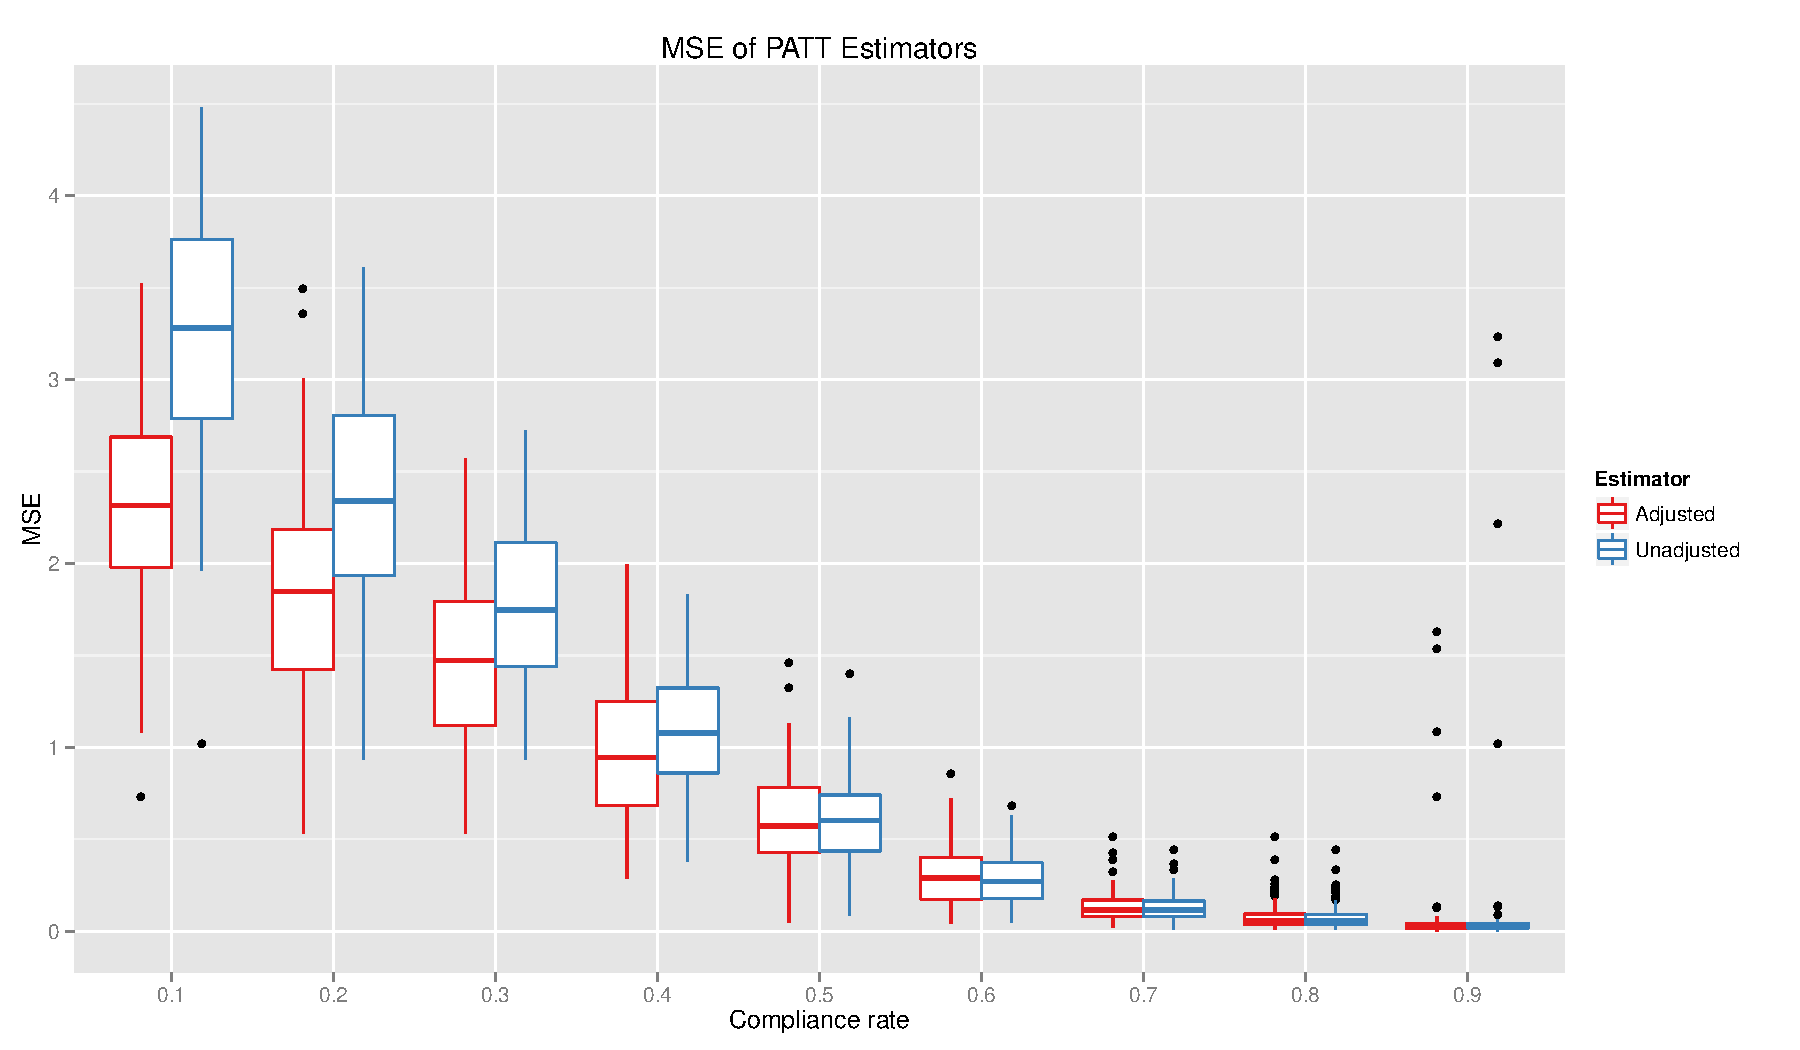
\includegraphics[width=\linewidth]{../paper/mse_boxplots_B5.pdf} 
 %  \footnotesize{Note: $p$ values are calculated using a two--sided randomization test ($\mathcal{L}=1,000$ iterations) for weighted difference of means between treatment and control groups. Refer to footnotes in Table \ref{balance-nom} and Figure \ref{qq} for variable descriptions.}
\label{simulation-plot}
\end{figure}
\end{frame}



\section[Application]{}

\begin{frame}
\frametitle{Application: Oregon Health Insurance Experiment (OHIE)}
\begin{itemize}
\item In 2008, $\approx$ 90,000 uninsured low-income adults participated in a lottery to receive Medicaid benefits \citep{finkelstein2012}
\item Participants selected by the lottery won the opportunity for themselves and any household member to apply for Medicaid
\item After sample exclusions, 29,834 participants were selected by the lottery; remaining 45,008 served as controls 
\item Two health care use responses from mail survey (N = 23,741): emergency room (ER) and primary care visits in past 12 months
\item Compliance measure: indicator for whether participant was enrolled in Medicaid program during study period
\end{itemize}
\end{frame}

\begin{frame}
\frametitle{Observational data}
\begin{itemize}
\item Data on the target population from National Health Interview Study (NHIS) \cite{NHIS} for 2009--2013
\item Restrict to respondents with income is below 138\% of the FPL
\item Covariates and responses match OHIE
\item OHIE compliance analogue: indicator for whether respondents are on Medicaid
\end{itemize}
\end{frame}

\begin{frame}
\frametitle{Checking Assumptions} % add to this
\begin{itemize}
\item Monotonicity is violated. There is some 2-way cross-over
\item Key assumption is strong ignorability: model of response given covariates is the same in the RCT and in the population
\begin{itemize}
\item No way to check that we've included all possible confounders
\item We have included all the confounders we have data on
\end{itemize}
\end{itemize}
\end{frame}

\begin{frame}
\frametitle{Checking Assumptions (cont.)}
{\scriptsize
\begin{longtable}{lllllll}
  & OHIE &  & OHIE &  & NHIS &  \\ 
    & control &  & treated &  &treated &   \\ 
  & $n=5104$ &  & $n=5193$ &  & $n=3914$ &  \\  
  \hline   
    \hline   
 \textbf{Covariate} &  $\mathbf{n}$ & $\mathbf{\%}$ & $\mathbf{n}$ & $\mathbf{\%}$ & $\mathbf{n}$ & $\mathbf{\%}$ \\ 
\hline
Female & 2970 & 58.2 & 2920 & 56.2 & 2712 & 69.3  \\ 
   \hline
20-49 & 1307 & 25.6 & 1367 & 26.3 & 1418 & 36.2  \\ 
   \hline
50-64 & 3797 & 74.4 & 3826 & 73.7 & 2496 & 63.8 \\ 
   \hline
White & 4420 & 86.6 & 4393 & 84.6 & 2308 & 59.0  \\ 
   \hline
Black & 227 & 4.5 & 197 & 3.8 & 1192 & 30.4  \\ 
   \hline
Hispanic & 331 & 6.5 & 476 & 9.2 & 1054 & 26.9  \\ 
   \hline
Diabetes & 518 & 10.2 & 539 & 10.4 & 689 & 17.6 \\ 
   \hline
Asthma & 986 & 19.3 & 887 & 17.1 & 748 & 19.1  \\ 
   \hline
High blood pressure & 1486 & 29.1 & 1418 & 27.3 & 1581 & 40.4  \\ 
   \hline
Heart condition & 159 & 3.1 & 141 & 2.7 & 396 & 10.1 \\ 
   \hline
Less than high school  & 994 & 19.5 & 950 & 18.3 & 1555 & 39.7  \\ 
   \hline
High school diploma or GED & 2908 & 57.0 & 2775 & 53.4 & 1193 & 30.5 \\ 
   \hline
Vocational training / 2-year degree & 922 & 18.1 & 1031 & 19.9 & 945 & 24.1 \\ 
   \hline
4-year college degree or more & 280 & 5.5 & 437 & 8.4 & 221 & 5.7 \\ 
   \hline
\hline
 \textbf{Response} &   &  &  & &  &  \\ 
Any ER visit & 1289 & 25.2 & 1323 & 25.5 & 860 & 22.0  \\ 
   \hline
\hline
Any primary care visit & 3044 & 59.6 & 3125 & 60.2 & 3175 & 81.1 \\ 
\hline
\hline
%\caption{Pretreatment covariates and responses for the OHIE and for NHIS respondents who received Medicaid.} 
\label{rct-nrt-compare}
\end{longtable}
}
\end{frame}


\begin{frame} % This slide is too wordy
\frametitle{Estimation Procedure}
\begin{enumerate}
\item Using the Medicaid lottery winners in the OHIE $(S=1, T=1)$, train a model to predict complier status using observed covariates.
\item Predict which lottery losers in the OHIE \textit{would have} signed up for Medicaid had they been eligible.
\item For the group of observed compliers to treatment and predicted compliers in the control group, train a model to predict hospital use using the covariates and Medicaid enrollment as features. 
\item For all individuals who enrolled in Medicaid in the NHIS, estimate their potential outcomes $Y_{10}$ and $Y_{11}$ using the model from step 3.  The mean counterfactual $Y_{11}$ minus the mean counterfactual $Y_{10}$ is the estimate of $\tau_{\text{PATT}}$.
\end{enumerate}
\end{frame}



\section[Results]{}

\begin{frame}
\begin{figure}[htbp]
\begin{center}
       \caption{Any ER visit.}
   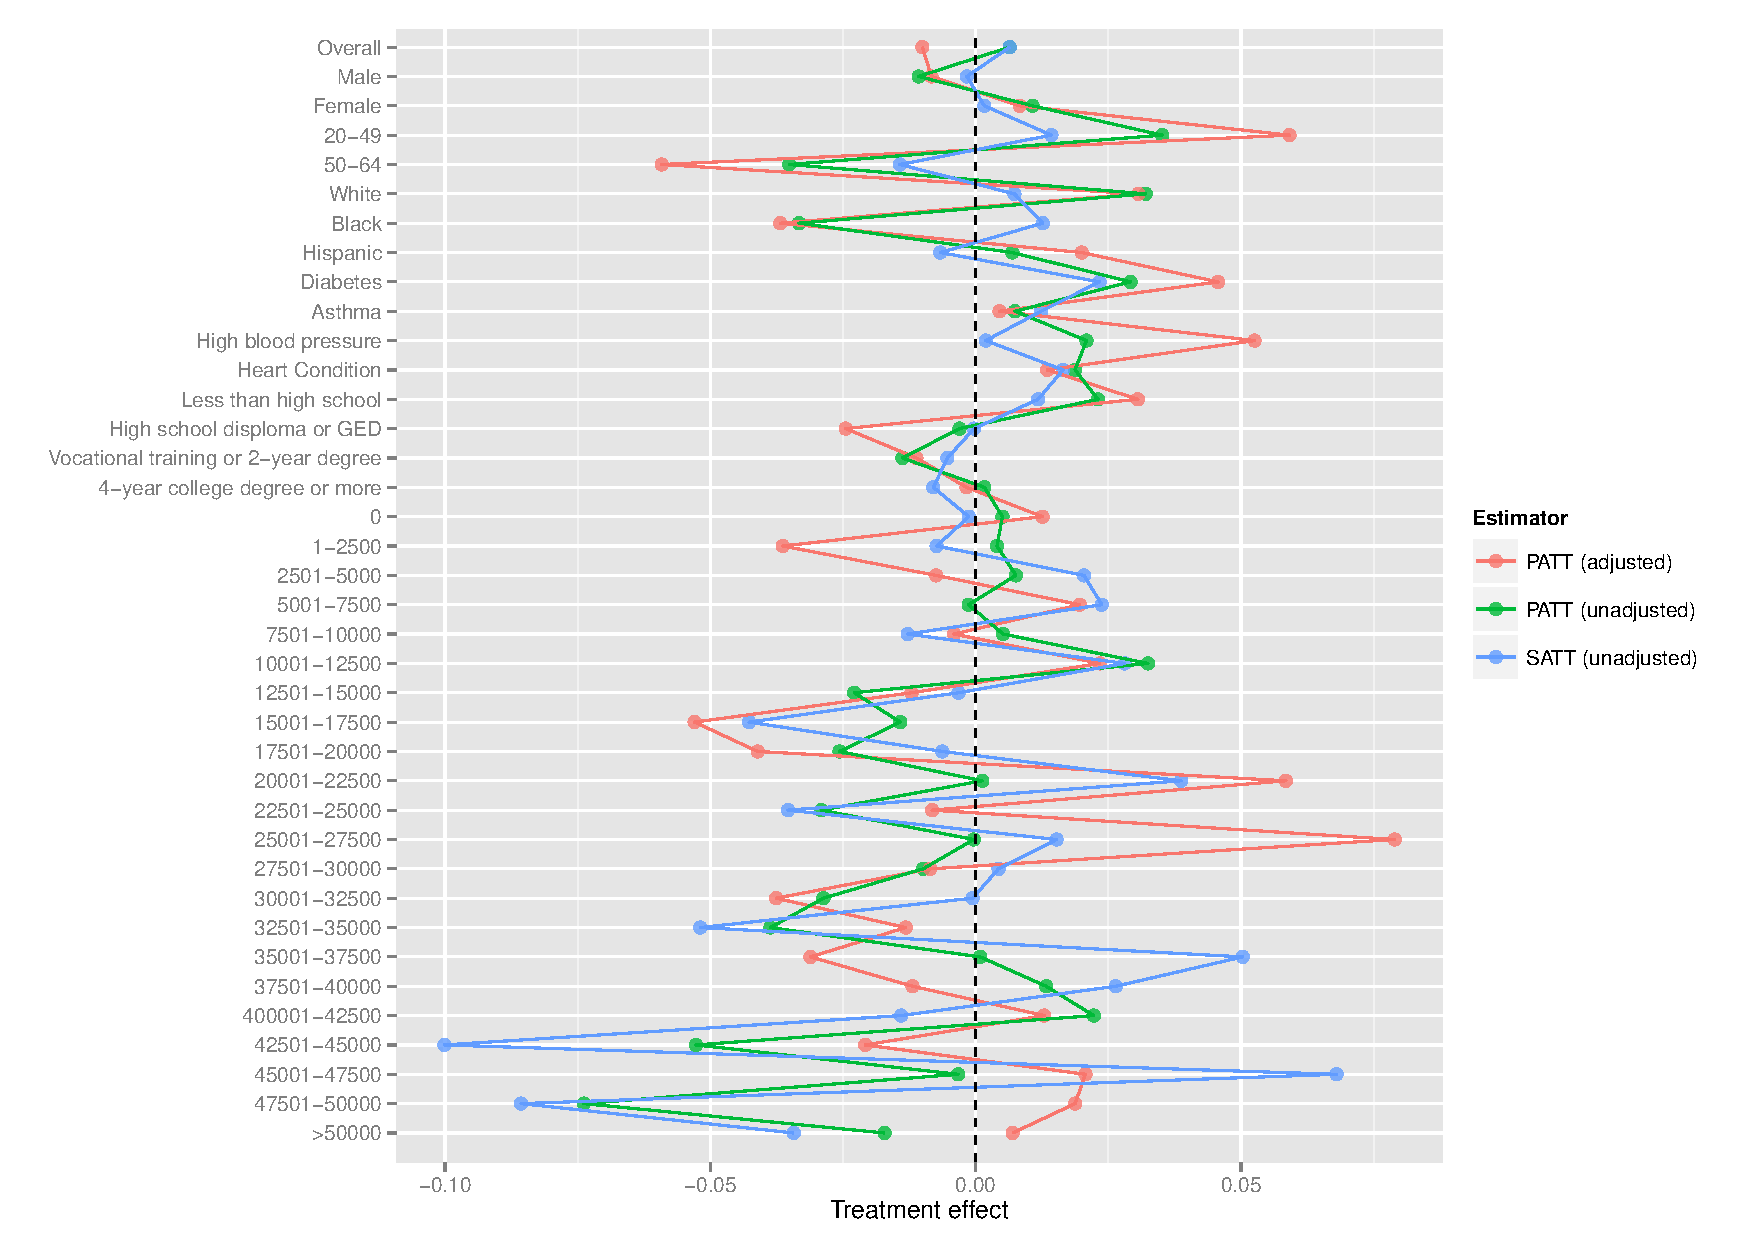
\includegraphics[scale=0.35]{../paper/any-visit-plot.pdf} 
   \label{het-plot-av}
   \end{center}
\end{figure}
\end{frame}

\begin{frame}
\begin{figure}[htbp]
\begin{center}
    \caption{Any primary care visit.}
   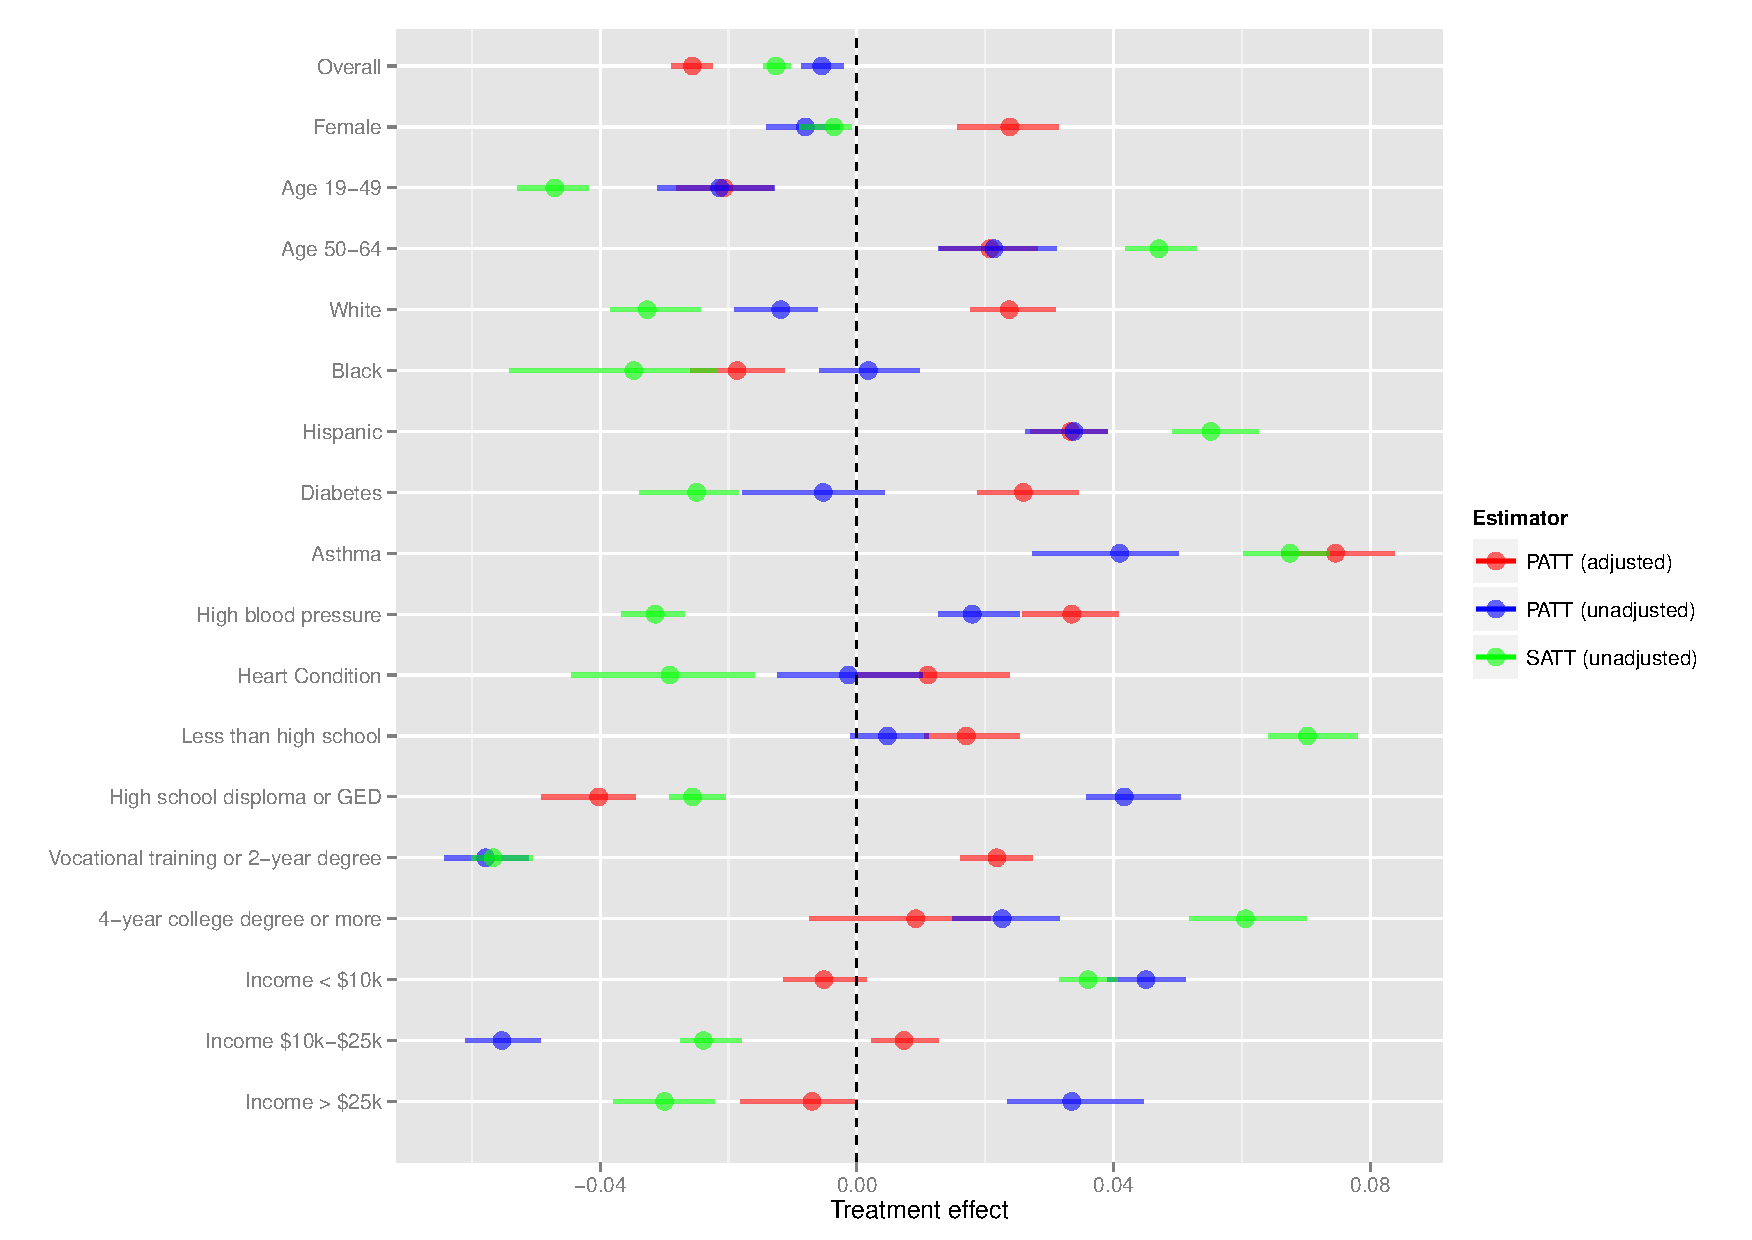
\includegraphics[scale=0.35]{../paper/any-out-plot.pdf} 
   \label{het-plot-ao}
   \end{center}
\end{figure}
\end{frame}



\section[Conclusions]{}

\begin{frame}
\frametitle{Conclusions}
\begin{itemize}
\item If the compliance rate is moderate and compliance is predictable by observed covariates, then it makes sense to use the proposed estimator % wording
\item statement or two about the OHIE/NHIS conclusions
\end{itemize}
\end{frame}

\section[References]{}

\begin{frame}
\begin{singlespace}
\begin{tiny}
\bibliographystyle{plainnat}
\bibliography{../paper/refs}
\end{tiny}
\end{singlespace}
\itemize
\end{frame}

		
\end{document}

